% !TEX root = paper.tex

\documentclass[11pt,letterpaper]{article}

% Packages
\usepackage{packages}
\addbibresource{sources.bib}

% Document Settings
\geometry{margin=1in}
\setlength{\parskip}{1ex}
\setlength{\parindent}{0pt}

\pagestyle{fancy}
\lhead{Väinö-verneri Kauppila} % controls the left corner of the header
\chead{} % controls the center of the header
\rhead{} % controls the right corner of the header
\lfoot{} % controls the left corner of the footer
\cfoot{} % controls the center of the footer
\rfoot{Page~\thepage} % controls the right corner of the footer
\renewcommand{\headrulewidth}{0.4pt}
\renewcommand{\footrulewidth}{0.4pt}

% =========================================
%             DOCUMENT
% =========================================

\begin{document}
\doublespacing % Double spacing throughout the document


% =========================
%      TITLE PAGE
% =========================

% Suppresses headers, footers, and page numbers on title page
\begin{titlepage}
    \begin{center}
        \vspace*{4cm}
        A statistical approach to predicting a tsunami’s wave height \\
        \vspace{1cm}
        Can the height of a tsunami's wave be predicted based on the distance from and
        the magnitude of a preceding earthquake? \\
        \vspace{1cm}
        \textit{Väinö-verneri Kauppila} \\
        February 2021 \\
        \vspace{4cm}
        Word count: TBD
        \vfill
        \vspace{0.1cm}
    \end{center}
\end{titlepage}

% =========================
%      DOCUMENT BODY
% =========================

\pagenumbering{roman}

\begin{center}
    \pdfbookmark{\contentsname}{Contents}
    \tableofcontents
    \vspace{1in}

\end{center}


% TODO: Add hyper-references to links
% TODO: Improve listings' styling
% TODO: Add links to Contents entries

\newpage

\pagenumbering{arabic}

\section{Introduction}

\subsection{Background}

Naturally occurring disasters, such as tsunamis, are devastating for people, human settlements, 
buildings and other resources residing in risk areas. Tsunamis are caused
by many different types of natural phenomena, such as landslides, collapse of
seamount, or more rarely, the impact of a meteorite. This paper, however, focuses
on one of the more common causes of tsunamis; earthquakes. Earthquakes cause around 72\% 
of tsunamis \cite{pacifictsunamimuseum}. The time between an earthquake and its tsunami is 
relatively long compared to events such as landslides \cite{sue_nokes_walters},
leaving adequate time to prepare for impact. Predicting wave height, as discussed in this 
paper, can further help to assess the seriousness of the tsunami and provide help to 
prepare for the event.

\subsection{Personal Engagement}

I have chosen to write about this subject as I have recently become interested by the
statistics and its implications in real-life matters. This research has proved very
interesting for me as it has made the field of statistics more concrete, because it provides 
a real world use case. Furthermore, as I enjoy programming, the research I have done 
has helped me learn about the tools and techniques used by data analysts and other professionals.

\section{Statistical Model}

\subsection{Processing the dataset for use}
%TODO: #2 Ask for help 
The dataset, procured from the NOAA website \cite{noaa}, includes many tsunami
runups, going back before the year 0. Due to this, the NOAA states uncertainties
that can occur in its data. For example, reports that were recorded before the
20th century tend to be based on written accounts, and not recorded seismic activity.
Only since the 1960s, the installation of the Worldwide Standardized Seismograph
Network system allowed for more accurate data in this paper. For that reason, any recorded
activity before this date was discarded from the dataset for this paper. The dataset itself can
be accessed through two different methods; searching the database using the online
tool or downloading it in a somewhat obscure compressed Google Earth \verb|.kmz| format. 
The online tool supports the download of search results in a much more human-readable 
\verb|.csv| format. For this paper, all entries after the year 1900 were searched and downloaded.

The data is cleaned of data points marked as "dubious" (there is an column for this parameter), 
reports before the year 1960 (see above), and of all irrelevant fields such as "Injuries" 
or "Damage \$Mil". This preliminary data cleanup
is done through the use of the pandas Python library \cite{reback2020pandas}\cite{mckinney-proc-scipy-2010}, 
which is commonly used for the handling of large datasets for its efficiency. 

The data was split into a training and a test dataset. The training
dataset was used to generate a regression model while the test dataset was used 
to calculate the general accuracy of the model, by predicting values and
comparing those to the known value as found in the dataset. The dataset was split based on
a fraction using the \verb|df.sample| method found in the pandas library. A split
of 70\% for training and 30\% for test was chosen. A \verb|random_state| argument is
set to an arbitrary value 42, as if it weren't, the dataset would be split in a different
manner at each execution of the program.

\subsection{Regression}

Regression analysis is a commonly used tool in statistics, and regression models can
be found in numerous use cases. Regression models consist of estimating the
relationship between one (or more) independent variables and a dependent variable. A
simple example of regression can be seen in the linear relationship between an independent
variable $x_{i}$, and the dependent variable $y$. The following expression shows this relationship in what is
called linear regression, as it models a straight line that can be used for prediction of 
values:

$y =  \beta_0 a + \beta_1 x + e $,

where the term $\beta_0$ represents the y-intercept of the line and $\beta$ represents the
coefficient of $x$. The final term $e$ is what is known as the error or residual
term. It is an estimate of the amount by which the predictions differ from the real
value.

However, the relationship between the distance between an earthquake and its tsunami 
and the wave height is not necessarily linear, especially if it is considered that the travel of
sound (which is a wave, or the displacement of a fluid that can travel) in a fluid obeys the 
inverse square law. Therefore, a simple linear regression model cannot be 
used for this research. A second degree polynomial regression formula would be more 
appropriate, and a new $x^2$ term can be added to the previous formula. We get:

$y = a + \beta_1 x + \beta_2 x^2 + e$

Even though the right side of this equation is quadratic in $x$, this is still
linear regression as the right side is linear in $\beta$ (if we were to let
$x = 1$, we would be left with $y = a + \beta_1 + \beta_2 + e$, which is linear).
A second degree polynomial regression would best fit our model for both independent
variables, as seen in the graphs below, where a theoretical curve of regression is drawn
by hand:

\begin{figure}[h]
    \centering
    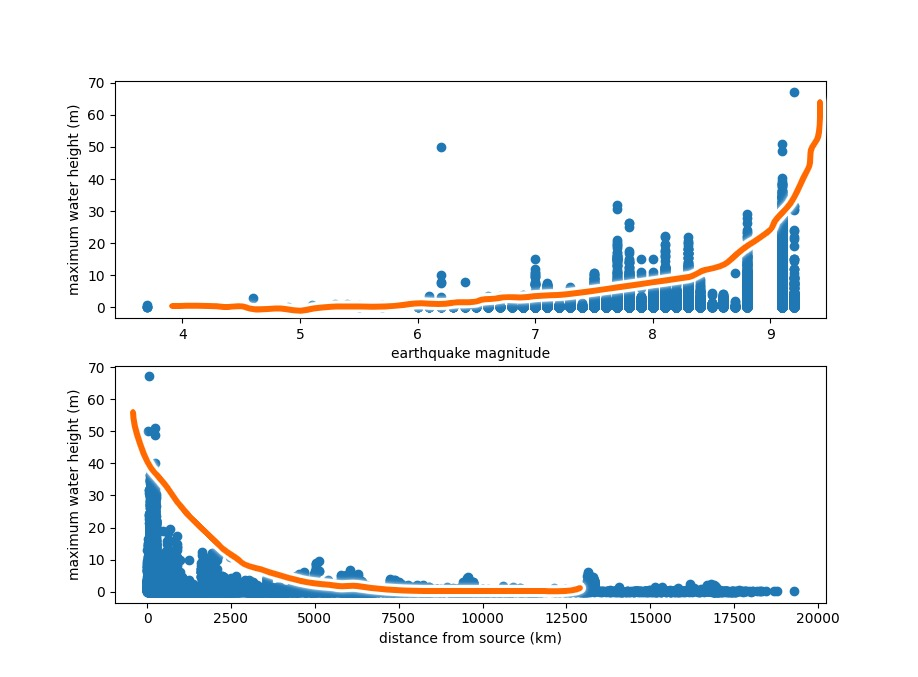
\includegraphics[width=0.6\textwidth]{modelshowcase.jpeg}
    \label{fig:boat1}
\end{figure}

In addition, our dataset has two independent variables: the distance from a particular
earthquake event and the magnitude of that earthquake. Models such as the one explored 
in this paper, where multiple independent variables are present, are called multivariate 
and can be modeled by adding the terms of a new independent variable, as such 
for a linear model with two independent variables:

$a_1 + \beta_1 x_1 + a_2 + \beta_2 x_2 + e$, 

where the terms $a_n$ are the y-intercepts of the $n$th independent variable, 


So the relationship between the two independent variables and the wave height can
be estimated with a multivariate, polynomial regression model. We will use the Python
scikit-learn library to aid in creating this model.

\begin{figure}[h]
    \centering
    \subfloat[\centering Linear model]{{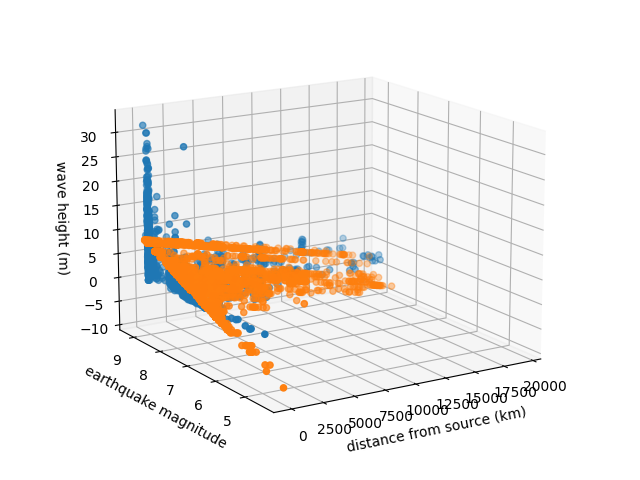
\includegraphics[width=5cm]{linear.png} }}
    \qquad
    \subfloat[\centering Polynomial model]{{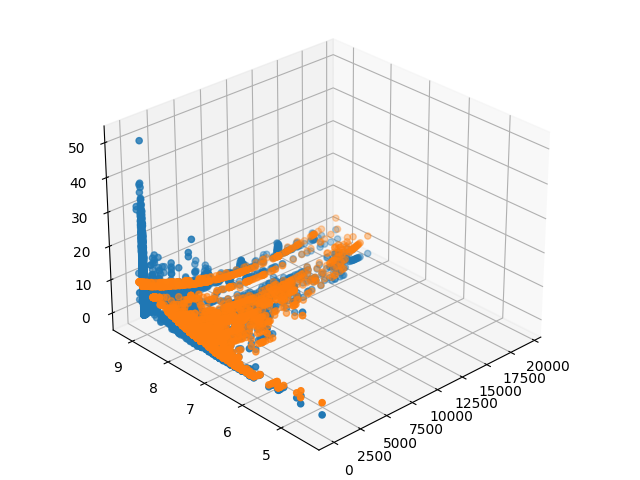
\includegraphics[width=5cm]{poly.png} }}
    \caption{2 multivariate (hence the 3 dimensions) regression models}
    \label{fig:example}
\end{figure}


\dots

The model's fit is then calculated, with the test dataset. The \verb|accuracy_score| method 
from the \verb|sklearn.metrics| class was used for this task. This function calculates what 
is called the $R^2$ value, which explains the extent at which the variance (the amount by which numbers 
are spread from the average value) in the dependent variable can be explained by the independent 
variable(s). An $R^2$ value of 0.6 indicates that 60\% of the model's results match those of the 
dataset. This value is defined as: 

$R^2 = 1 - \frac{SS_{res}}{SS_{total}}$,

where $SS_{res}$ is the sum of the error terms, or the residual sum of squares, in a dataset of $n$ 
values $y_1,\dots, y_i$, with their corresponding predicted values $p_1,\dots, p_i$ defined by 

$SS_{res} = \sum_{i} (y_i - p_i)^2 = \sum_{i} e_i^2$, \footnote{$\sum_i i$ would mean that all values i 
are summed} where $e_i$ is the error term, equal to the difference of a data point $y_i$ 
and its corresponding predicted value $p_i$.

and $SS_{tot}$ is the total sum of squares, which is proportional to the variance in the data, 
defined as:

$SS_{tot} = \sum_{i} (y_i - \bar y)^2$, where $\bar y$ is the mean of the data $y_1,\dots, y_i$, 
or $\bar y = \frac{1}{n} \sum_{i=1}^n y_i$

\section{Conclusion}

The research included in this paper could be useful for many life-saving scenarios,
notably ones in which, for example, high quality and large-scale tsunami alert
systems are not available.

\subsection{Evaluation of the method used}

This method, like any other statistical approximation, is by no means perfect
and for that reason should not be used in any real-world application. The results
procured by the program are subject to many uncertainties, one of which is described
below.

When attempting to predict the maximum wave height of a tsunami such as the one
caused by the 2011 earthquake off the Pacific coast of Tōhoku, approximately 70km
away from shore, which produced a 38.9m wave \cite{yomiuri_2011}. The model in this
paper approximates this same event as only a 8m wave, when supplied the 9.0 magnitude
of the earthquake and the 70km distance. These types of errors can be attributed to the
fact that there are many more independent variables, such as the shape of the seafloor for
example, that can amplify or potentially change the height of a tsunami's wave.


\printbibliography[heading=bibintoc, title=Works Cited]

\appendix
\section{Appendix}
\label{app}
\subsection{Python program}
\label{app:scripts}

Listed here is the Python program through which the dataset was cleaned and
predictions based on the statistical model were made. Run using 64-bit Python
version 3.9.1.

\lstinputlisting[language=Python]{model/multregr2.py}


\end{document}